\subsection{Determining upper and lower bound support}

Because the total number of possible rules extracted
from a data set grows exponentially, it is necessary to find determine an appropriate value of minimum support count. This is to avoid wasting computational power in finding uninteresting and obvious rules.
Hence, the best rules should have \textit{relatively} low support and high confidence.
We run the apriori algorithm and let weka generate output itemsets for us.  We copy the one itemset frequency list into excel and generate the following table.
A 1-itemset frequency list is generated by running the Apriori algorithm in Weka with
\begin{verbatim}
	 weka.associations.Apriori -I -N 1000 -T 0 -C 0.9 -D 0.05 -U 1.0 -M 0.1 -S -1.0 -c -1
\end{verbatim}
The support of the frequent 1-itemsets (with a lower bound $minsup = 0.1$) is shown in the figure below.

\begin{figure}[H]
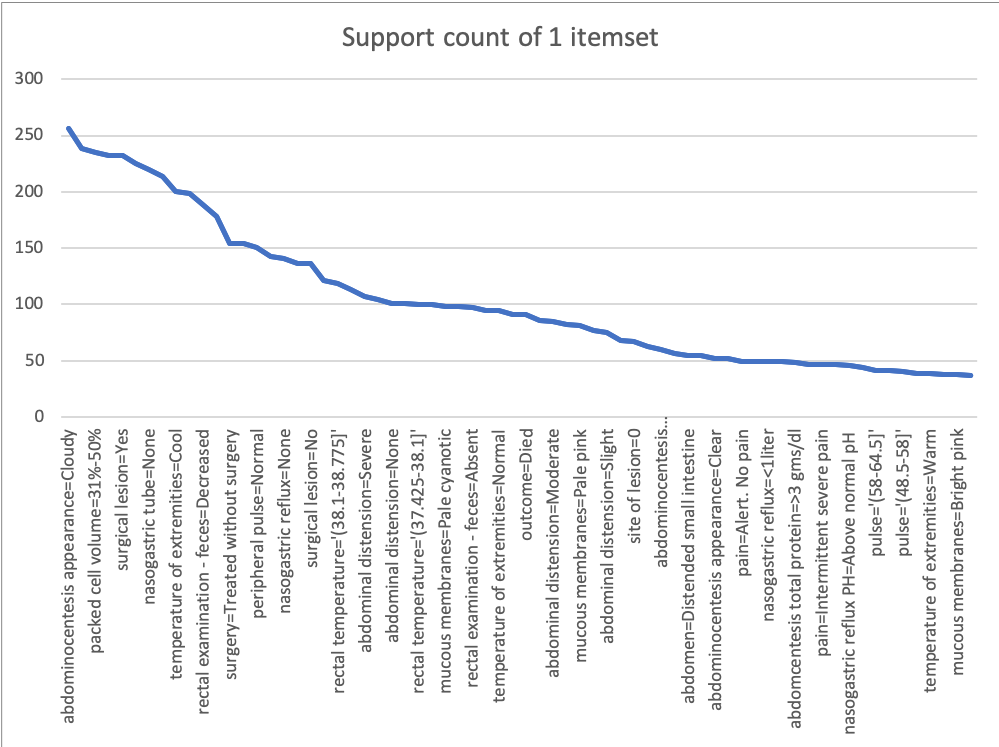
\includegraphics[scale=0.7]{SupportCountTable.png}

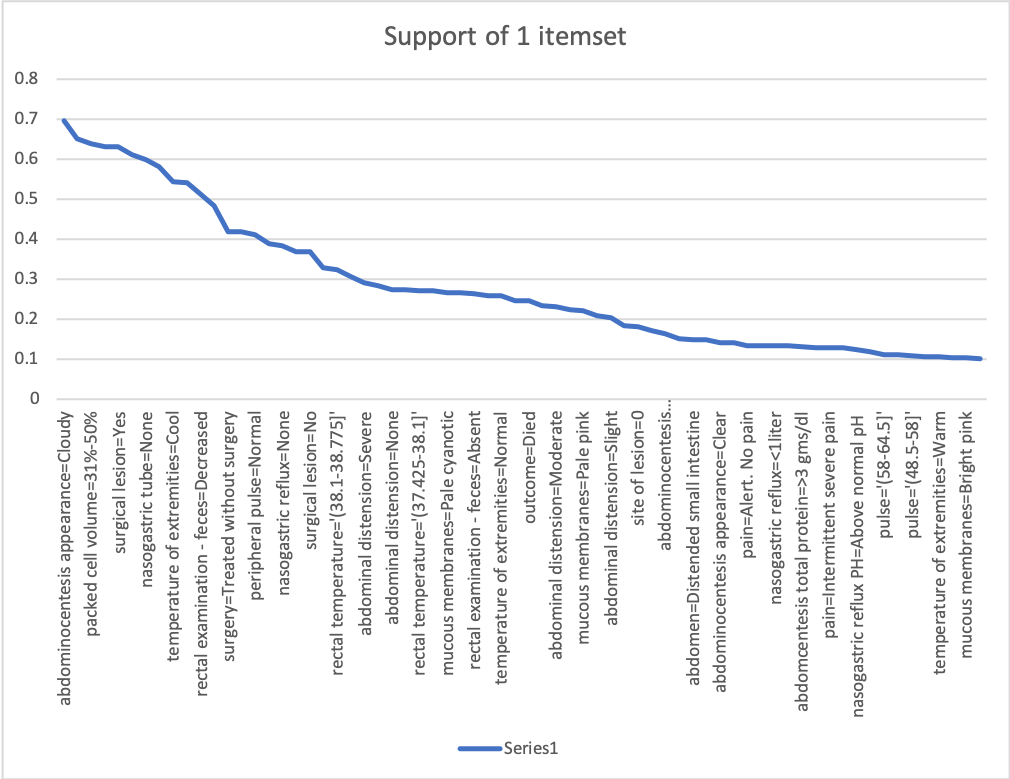
\includegraphics[scale=0.7]{SupportTable.png}
\end{figure}

\noindent
From the table, one can deduce that the most interesting rules will have support level of less than 0.42 since any rule with more support than that will probably be rather obvious. So we set the upperBoundMinSupport to 0.42 in the Associate settings.\\
As computational resources are limited, lowerBoundMinSupport is set to 0.1.